\section{Durchführung}
\label{sec:Durchführung}

Zunächst haben wir die Leerlaufspannung der Monozelle unmittelbar gemessen und
den angegebenen Eingangswiderstand $R_\text{V}$ notiert.

Dann haben wir bei variablem Belastungsstrom $I$ die Klemmenspannung $U_\text{K}$
aufgenommen. Um den Strom zu variieren haben wir den Belastungswiderstand variiert.
Dazu wurde Schaltung \ref{fig:Schaltung1} verwendet.

\begin{figure}[h]
  \centering
  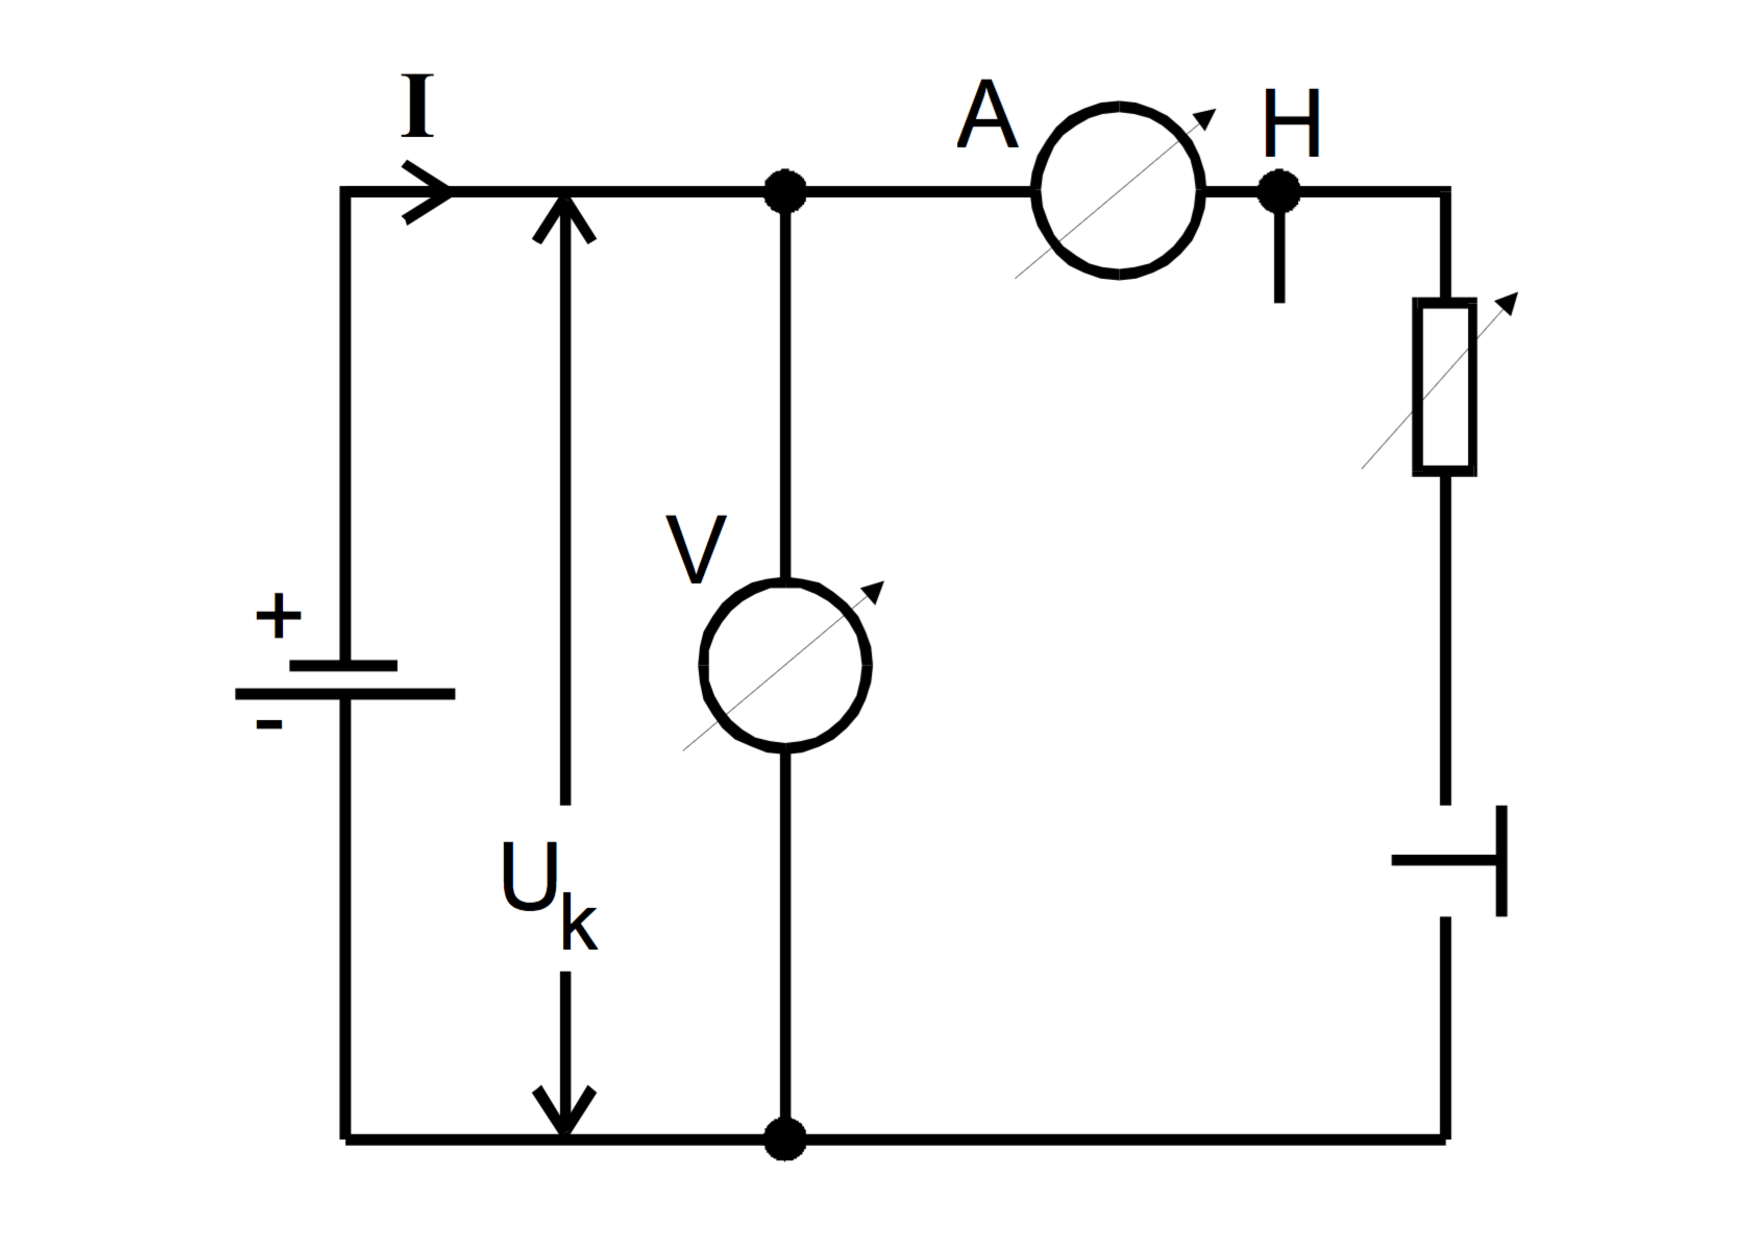
\includegraphics[height = 5cm]{Abbildung 1.pdf}
  \caption{Messschaltung 1 zum Messen an der Monozelle.}
  \label{fig:Schaltung1}
\end{figure}

Danach haben wir eine Gegenspannung in die Schaltung eingebaut, die den Strom
in die entgegengesetzte Richtung fließen ließ. Hier ändert sich die Klemmenspannung
wie in Gleichung \eqref{eqn:Gegenspannung}.

\begin{equation}
  U_\text{K} = U_\text{0} + IR_\text{i}
  \label{eqn:Gegenspannung}
\end{equation}

Es wurden aber erneut $U_\text{K}$ und $I$ aufgenommen. Abbildung \ref{fig:Schaltung2}
zeigt die verwendete Schaltung.

\begin{figure}[h]
  \centering
  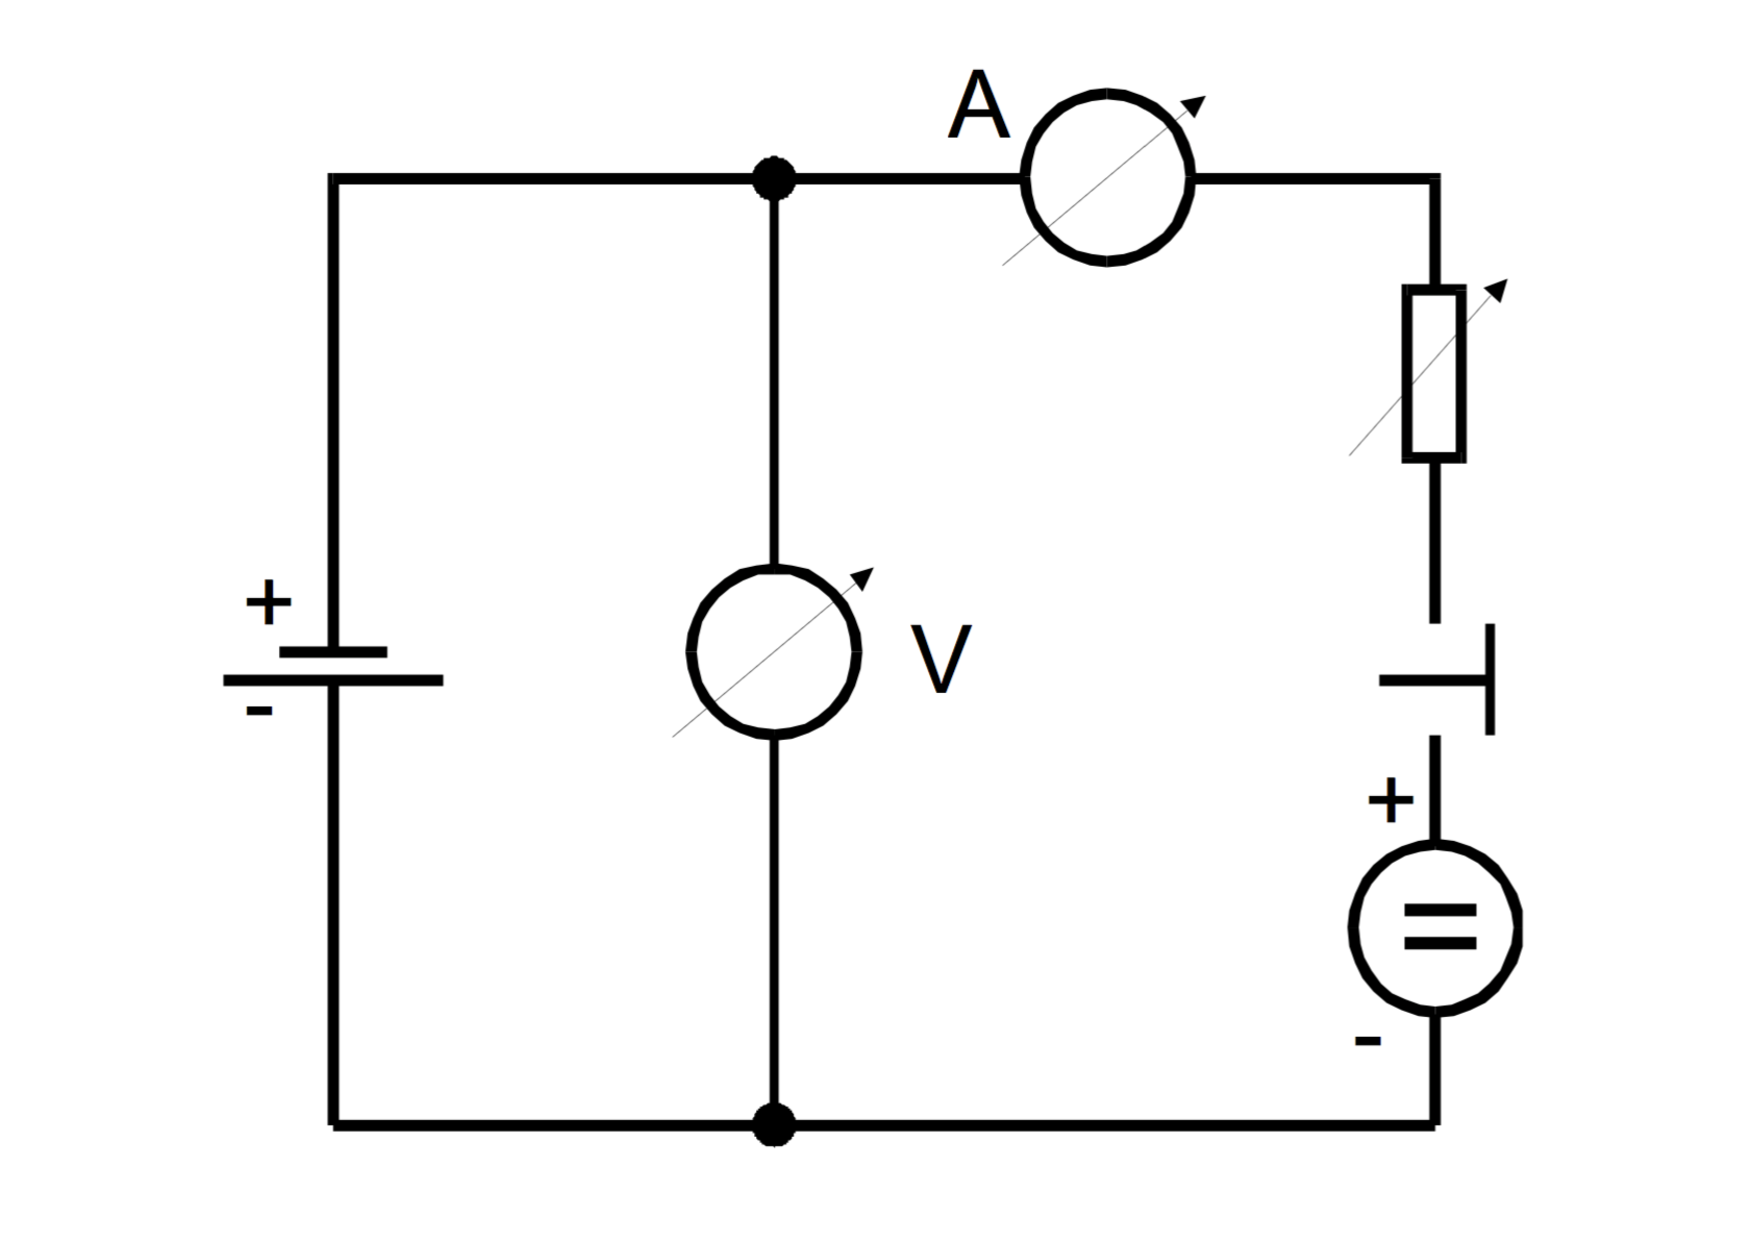
\includegraphics[height = 5cm]{Abbildung 2.pdf}
  \caption{Messschaltung 2 mit der Gegenspannung.}
  \label{fig:Schaltung2}
\end{figure}

Zuletzt haben wir die Messung aus Schritt 2 widerholt; allerdings mit dem Sinus-
und Rechteckausgang eines RC-Generators als Messobjekt.
Die Schaltungen mit dem Rechteck- und Sinusausgang als Messobjekte werden im
Folgenden mit 3a beziehungsweise mit 3b bezeichnet.
